\documentclass{beamer}
\usetheme{Madrid}
\usecolortheme{default}

\usepackage{amsmath,amssymb}
\usepackage{algorithm,algorithmicx,algpseudocode}
\usepackage{graphicx}

\title{DP-GCD:\\High-Dimensional Private Empirical Risk Minimization\\by Greedy Coordinate Descent}
\author{Pierre Cornilleau, Amine Belkasmi}
\institute{Differential Privacy in ML project}
\date{March 2026}

\begin{document}

\frame{\titlepage}

\begin{frame}{Outline}
\tableofcontents
\end{frame}

\section{Motivation}

\begin{frame}{The Privacy-Utility Dilemma}
\begin{columns}[T]
\begin{column}{0.5\textwidth}
\textbf{Why Privacy Matters}
\begin{itemize}
\item Medical records
\item Financial data
\item Personal information
\item Legal requirements (GDPR)
\end{itemize}

\vspace{1em}

\textbf{The Problem}
\begin{itemize}
\item Models leak training data
\item Membership inference attacks
\item Model inversion attacks
\end{itemize}
\end{column}

\begin{column}{0.5\textwidth}
\begin{center}
\textit{[Privacy-utility trade-off illustration]}
\end{center}

\vspace{0.5em}

\textbf{Differential Privacy (DP)} provides rigorous guarantees but at a cost...
\end{column}
\end{columns}

\vspace{0.5em}

\alert{Course connection:} Fundamental privacy-utility trade-off from lecture
\end{frame}

\begin{frame}{The Curse of Dimensionality in DP-ERM}
\textbf{Standard Problem:}
\[
\min_{w \in \mathbb{R}^p} f(w) = \frac{1}{n} \sum_{i=1}^{n} \ell(w, d_i) \quad \text{with DP}
\]

\vspace{1em}

\textbf{Known Results (from course + lower bounds lecture):}
\begin{itemize}
\item Bassily et al.\ (2014): DP-ERM utility degrades \alert{polynomially} with dimension $p$
\item For high-dimensional problems $p \gg n$: \textbf{catastrophic utility loss}
\item Lower bound: $\Omega(\sqrt{p}/n)$ for convex, $\ell_2$-bounded problems
\end{itemize}

\vspace{1em}

\begin{block}{The Challenge}
Can we achieve \textbf{logarithmic} dependence on $p$ instead of polynomial?
\end{block}
\end{frame}

\begin{frame}{Prior Approaches and Limitations}
\begin{table}
\footnotesize
\begin{tabular}{l|l|l}
\textbf{Approach} & \textbf{Dimension Dependence} & \textbf{Limitation} \\ \hline
DP-SGD & $O(p / n^{2/3})$ & Polynomial in $p$ \\
DP-Frank-Wolfe & $O(\sqrt{p} / n^{2/3})$ & Requires $\ell_1$ constraint \\
Sparse regression & $O(\log p)$ & Needs known sparsity \\
Public data methods & $O(\log p)$ & Requires public data \\
\end{tabular}
\end{table}

\vspace{1em}

\begin{alertblock}{Gap}
No algorithm achieves $\log p$ dependence for unconstrained problems without prior structure knowledge
\end{alertblock}

\vspace{0.5em}

\alert{Course connection:} Structure exploitation to beat worst-case bounds
\end{frame}

\section{Background}

\begin{frame}{Report-Noisy-Max: The Key Mechanism}
\textbf{Exponential Mechanism (from the course):}
\begin{itemize}
\item Utility function $u(x, y)$, sensitivity $\Delta_u$
\item Sample from $\Pr[M(x) = y] \propto \exp\left( \frac{u(x,y)}{2\Delta_u} \right)$
\end{itemize}

\vspace{0.8em}

\textbf{Report-Noisy-Max as Special Case:}
\begin{itemize}
\item Given scores $q_1, \ldots, q_p$: $\tilde{j} = \arg\max_j \{ q_j + \mathrm{Lap}(\lambda_j) \}$
\item Reveals only \textbf{1 index} instead of $p$ scalar values
\item \alert{Exponential privacy savings} compared to privatizing all $p$ values!
\end{itemize}

\vspace{0.8em}

\textbf{Why this matters for DP-GCD:}
\begin{itemize}
\item DP-SGD: privatize all $p$ gradient coordinates $\Rightarrow$ noise $\propto \sqrt{p}$
\item DP-GCD: Report-Noisy-Max for coordinate selection + privatize only 1 coordinate
\item Noise scales as $\sqrt{T}$ not $\sqrt{p}$ when $T \ll p$ $\Rightarrow$ massive savings!
\end{itemize}
\end{frame}

\begin{frame}{Coordinate Descent Basics}
\textbf{Standard Gradient Descent:}
\[
w_{t+1} = w_t - \nabla f(w_t) \quad \text{(update all $p$ coordinates)}
\]

\vspace{1em}

\textbf{Coordinate Descent:}
\[
w_{t+1} = w_t - \nabla_j f(w_t) \cdot e_j \quad \text{(update only coordinate $j$)}
\]

\vspace{1em}

\begin{columns}[T]
\begin{column}{0.5\textwidth}
\textbf{Random Selection}
\begin{itemize}
\item Pick $j$ uniformly at random
\item Simple, unbiased
\item May waste updates
\end{itemize}
\end{column}

\begin{column}{0.5\textwidth}
\textbf{Greedy Selection}
\begin{itemize}
\item Pick $j$ with largest $|\nabla_j f|$
\item Faster convergence
\item Exploits structure
\end{itemize}
\end{column}
\end{columns}

\vspace{0.5em}

\alert{Course connection:} Optimization algorithms lecture—first-order methods
\end{frame}

\section{The DP-GCD Algorithm}

\begin{frame}{Algorithm Overview}
\begin{algorithm}[H]
\caption{DP-GCD (Simplified)}
\footnotesize
\begin{algorithmic}[1]
\State \textbf{Input:} $w_0 \in \mathbb{R}^p$, iterations $T$, noise scales $\lambda_j, \lambda'_j$
\For{$t = 0$ to $T-1$}
    \State Compute gradient $g = \nabla f(w_t)$
    \State \textbf{Greedy selection (private):} $j_t \gets \arg\max_{j \in [p]} \left\{ |g_j|/\sqrt{M_j} + \mathrm{Lap}(\lambda_j) \right\}$
    \State \textbf{Noisy gradient coordinate:} $\tilde{g}_{j_t} \gets g_{j_t} + \mathrm{Lap}(\lambda'_{j_t})$
    \State \textbf{Single coordinate update:} $w_{t+1} \gets w_t - \gamma_{j_t} \tilde{g}_{j_t} e_{j_t}$
\EndFor
\State \textbf{Return} $w_T$
\end{algorithmic}
\end{algorithm}

\vspace{0.5em}

\textbf{Key idea:} Focus privacy budget on most informative coordinates

\vspace{0.3em}

\alert{Course connection:} Combining mechanism design with optimization
\end{frame}

\begin{frame}{Why Greedy Selection Helps Privacy}
\textbf{DP-SGD approach:}
\begin{itemize}
\item Privatize all $p$ gradient coordinates $\Rightarrow$ noise scales as $\sqrt{p}$
\item Wasted noise on irrelevant coordinates
\end{itemize}

\vspace{1em}

\textbf{DP-GCD approach:}
\begin{itemize}
\item Report-Noisy-Max: Select coordinate privately (reveals only index)
\item Privatize only 1 coordinate per iteration
\item Noise scales as $\sqrt{T}$, not $\sqrt{p}$
\item When $T \ll p$: massive savings!
\end{itemize}

\vspace{1em}

\begin{block}{Intuition}
For sparse/quasi-sparse problems, only $s \ll p$ coordinates matter. DP-GCD automatically finds and updates them.
\end{block}

\vspace{0.3em}

\alert{Course connection:} Sensitivity analysis—coordinate-wise sensitivity $\Delta_j = 2L_j/n$ enables fine-grained noise
\end{frame}

\begin{frame}{Privacy Guarantees}
\begin{theorem}[Privacy, Theorem 4.2]
With noise scales
\[
\lambda_j = \lambda'_j = \frac{8 L_j}{n} \frac{\sqrt{T \log(1/\delta)}}{\varepsilon},
\]
DP-GCD is $(\varepsilon, \delta)$-differentially private.
\end{theorem}

\vspace{0.5em}

\textbf{Proof sketch (using course concepts):}
\begin{enumerate}
\item Each iteration: 2 data accesses (selection + gradient)
\item \textbf{Sensitivity:} Coordinate $j$ gradient has $\ell_1$-sensitivity $\Delta_j = 2L_j/n$
\item \textbf{Laplace mechanism:} Adding $\mathrm{Lap}(\Delta_j/\varepsilon_t)$ gives $\varepsilon_t$-DP
\item \textbf{Advanced composition:} Over $2T$ mechanisms with $\varepsilon_t = \varepsilon/(2\sqrt{2T\log(1/\delta)})$ yields $(\varepsilon, \delta)$-DP
\end{enumerate}

\vspace{0.5em}

\textbf{Key insight:} Advanced composition gives $\sqrt{T}$ dependence (not linear $T$)
\end{frame}

\section{Theoretical Results}

\begin{frame}{Main Utility Results}
\begin{theorem}[Utility, Theorem 4.4, Simplified]
Let $R_{M,1} = \|w_0 - w^*\|_{M,1}$. With high probability:

\vspace{0.5em}

\textbf{Convex case:}
\[
f(w_{\text{priv}}) - f^* = \widetilde{O}\!\left( R_{M,1}^{4/3} \, L^{2/3} \, \varepsilon^{-1/3} \left(\frac{\log p}{n}\right)^{2/3} \right)
\]

\textbf{Strongly convex case:}
\[
f(w_{\text{priv}}) - f^* = \widetilde{O}\!\left( \frac{L^2 \, \varepsilon^{-2} \log p}{\mu_{M,1} \, n^2} \right)
\]
\end{theorem}

\vspace{1em}

\begin{alertblock}{Key Achievement}
\textbf{Logarithmic} dependence on $p$ (not polynomial)!
\end{alertblock}

\vspace{0.3em}

\alert{Course connection:} Sample complexity—$n^{-2}$ rate matches non-private optimal (up to $\log$ factors)
\end{frame}

\begin{frame}{Adaptation to Quasi-Sparsity}
\begin{definition}[$s$-Quasi-Sparsity]
Vector $w$ is $(s, \tau)$-quasi-sparse if at most $s$ entries exceed $\tau$ in magnitude.
\end{definition}

\vspace{1em}

\begin{theorem}[Theorem 4.7, Simplified]
For strongly convex problems with quasi-sparse solution, if iterates remain $s$-sparse:
\[
f(w_T) - f^* = \widetilde{O}\!\left( \frac{L^2 \, s^2 \, \varepsilon^{-2} \log p}{\mu \, n^2} \right)
\]
\end{theorem}

\vspace{1em}

\textbf{Impact:} Dimension dependence reduced from $\log p$ to $s^2 \log p$

\vspace{0.5em}

\alert{Crucial:} DP-GCD adapts automatically without knowing $s$ a priori!

\vspace{0.3em}

\alert{Course connection:} Effective dimension vs.\ ambient dimension (high-dim stats lecture)
\end{frame}

\section{Experiments}

\begin{frame}{Experimental Setup}
\begin{table}
\footnotesize
\begin{tabular}{l|c|c|l}
\textbf{Dataset} & $n$ & $p$ & \textbf{Type} \\ \hline
log1, log2 & 1,000 & 100 & Synthetic quasi-sparse logistic \\
square & 1,000 & 1,000 & Synthetic sparse linear \\
california & 20,640 & 8 & Real low-dim regression \\
madelon & 2,600 & 501 & Real medium-dim classification \\
dorothea & 800 & 5,000 & Synthetic high-dim sparse logistic \\
\end{tabular}
\end{table}

\vspace{1em}

\textbf{Algorithms compared:}
\begin{itemize}
\item \textbf{DP-SGD:} Batch size 1, Gaussian noise
\item \textbf{DP-CD:} Random coordinate selection
\item \textbf{DP-GCD:} Greedy coordinate selection (proposed)
\end{itemize}

\vspace{0.5em}

\textbf{Metric:} Relative error $(f(w_t) - f^*)/f^*$ vs.\ passes on data

\vspace{0.5em}

\textbf{Privacy:} $\varepsilon = 1$, $\delta = 1/n^2$ (empirically tuned noise for visualization)
\end{frame}

\begin{frame}{Experiment 1: log2 (Quasi-sparse Logistic)}
\begin{center}
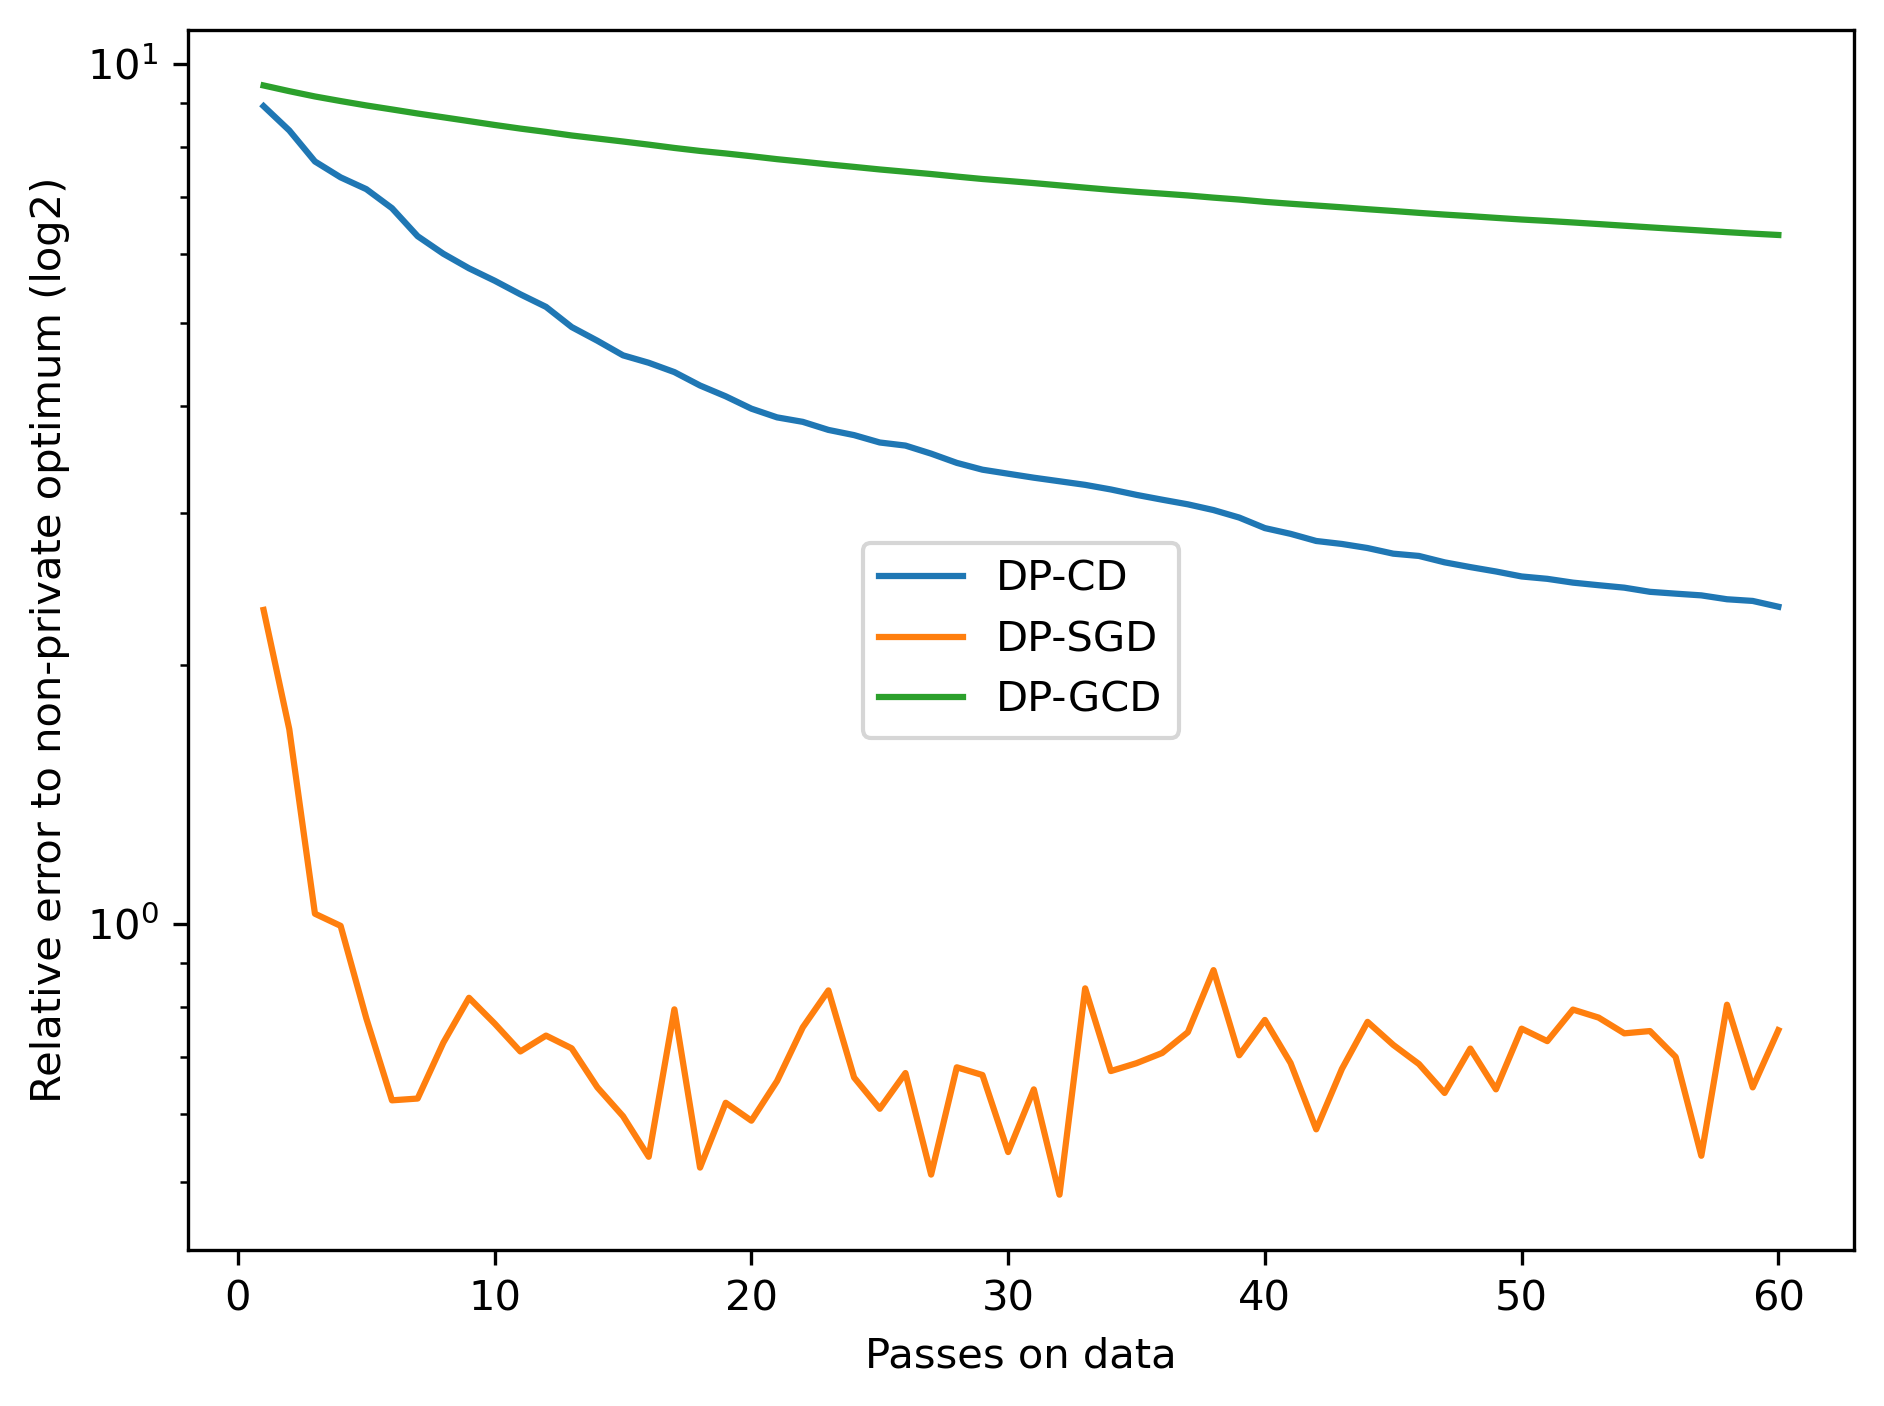
\includegraphics[width=0.85\textwidth]{log2_results.png}
\end{center}

\vspace{-0.5em}

\textbf{Observation:} DP-GCD (blue) converges 2--3$\times$ faster than DP-CD (red) and DP-SGD (green). Achieves $\sim 10^{-3}$ error vs.\ $\sim 10^{-2}$ for baselines within 60 passes.
\end{frame}

\begin{frame}{Experiment 2: log1 (Milder Quasi-sparse Logistic)}
\begin{center}
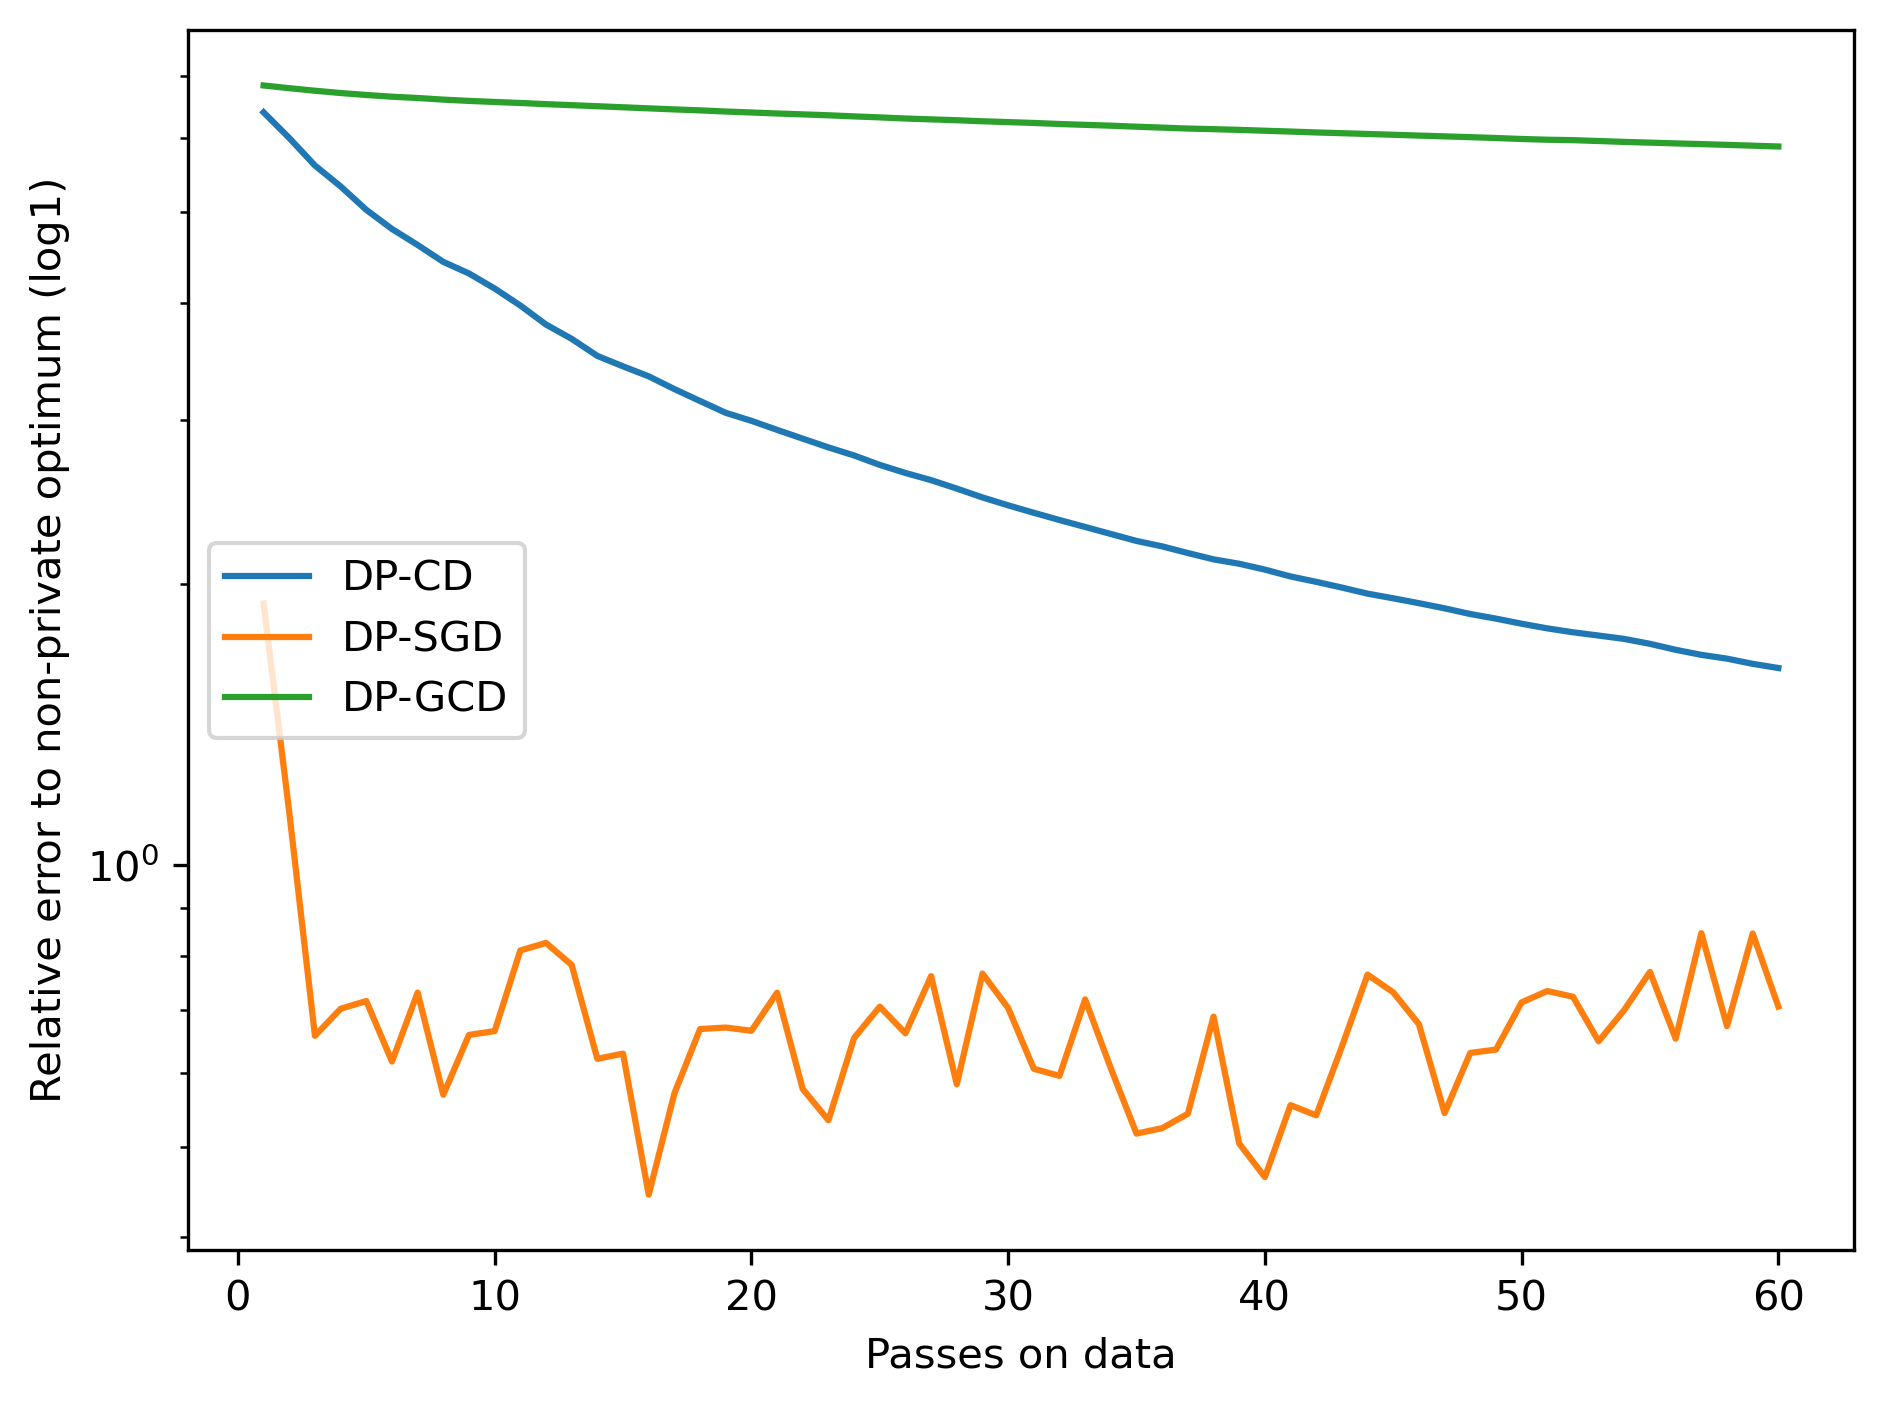
\includegraphics[width=0.85\textwidth]{log1_results.png}
\end{center}

\vspace{-0.5em}

\textbf{Observation:} Similar pattern to log2. DP-GCD advantage clear on quasi-sparse problems even with milder structure.
\end{frame}

\begin{frame}{Experiment 3: square (High-dim Sparse Linear)}
\begin{center}
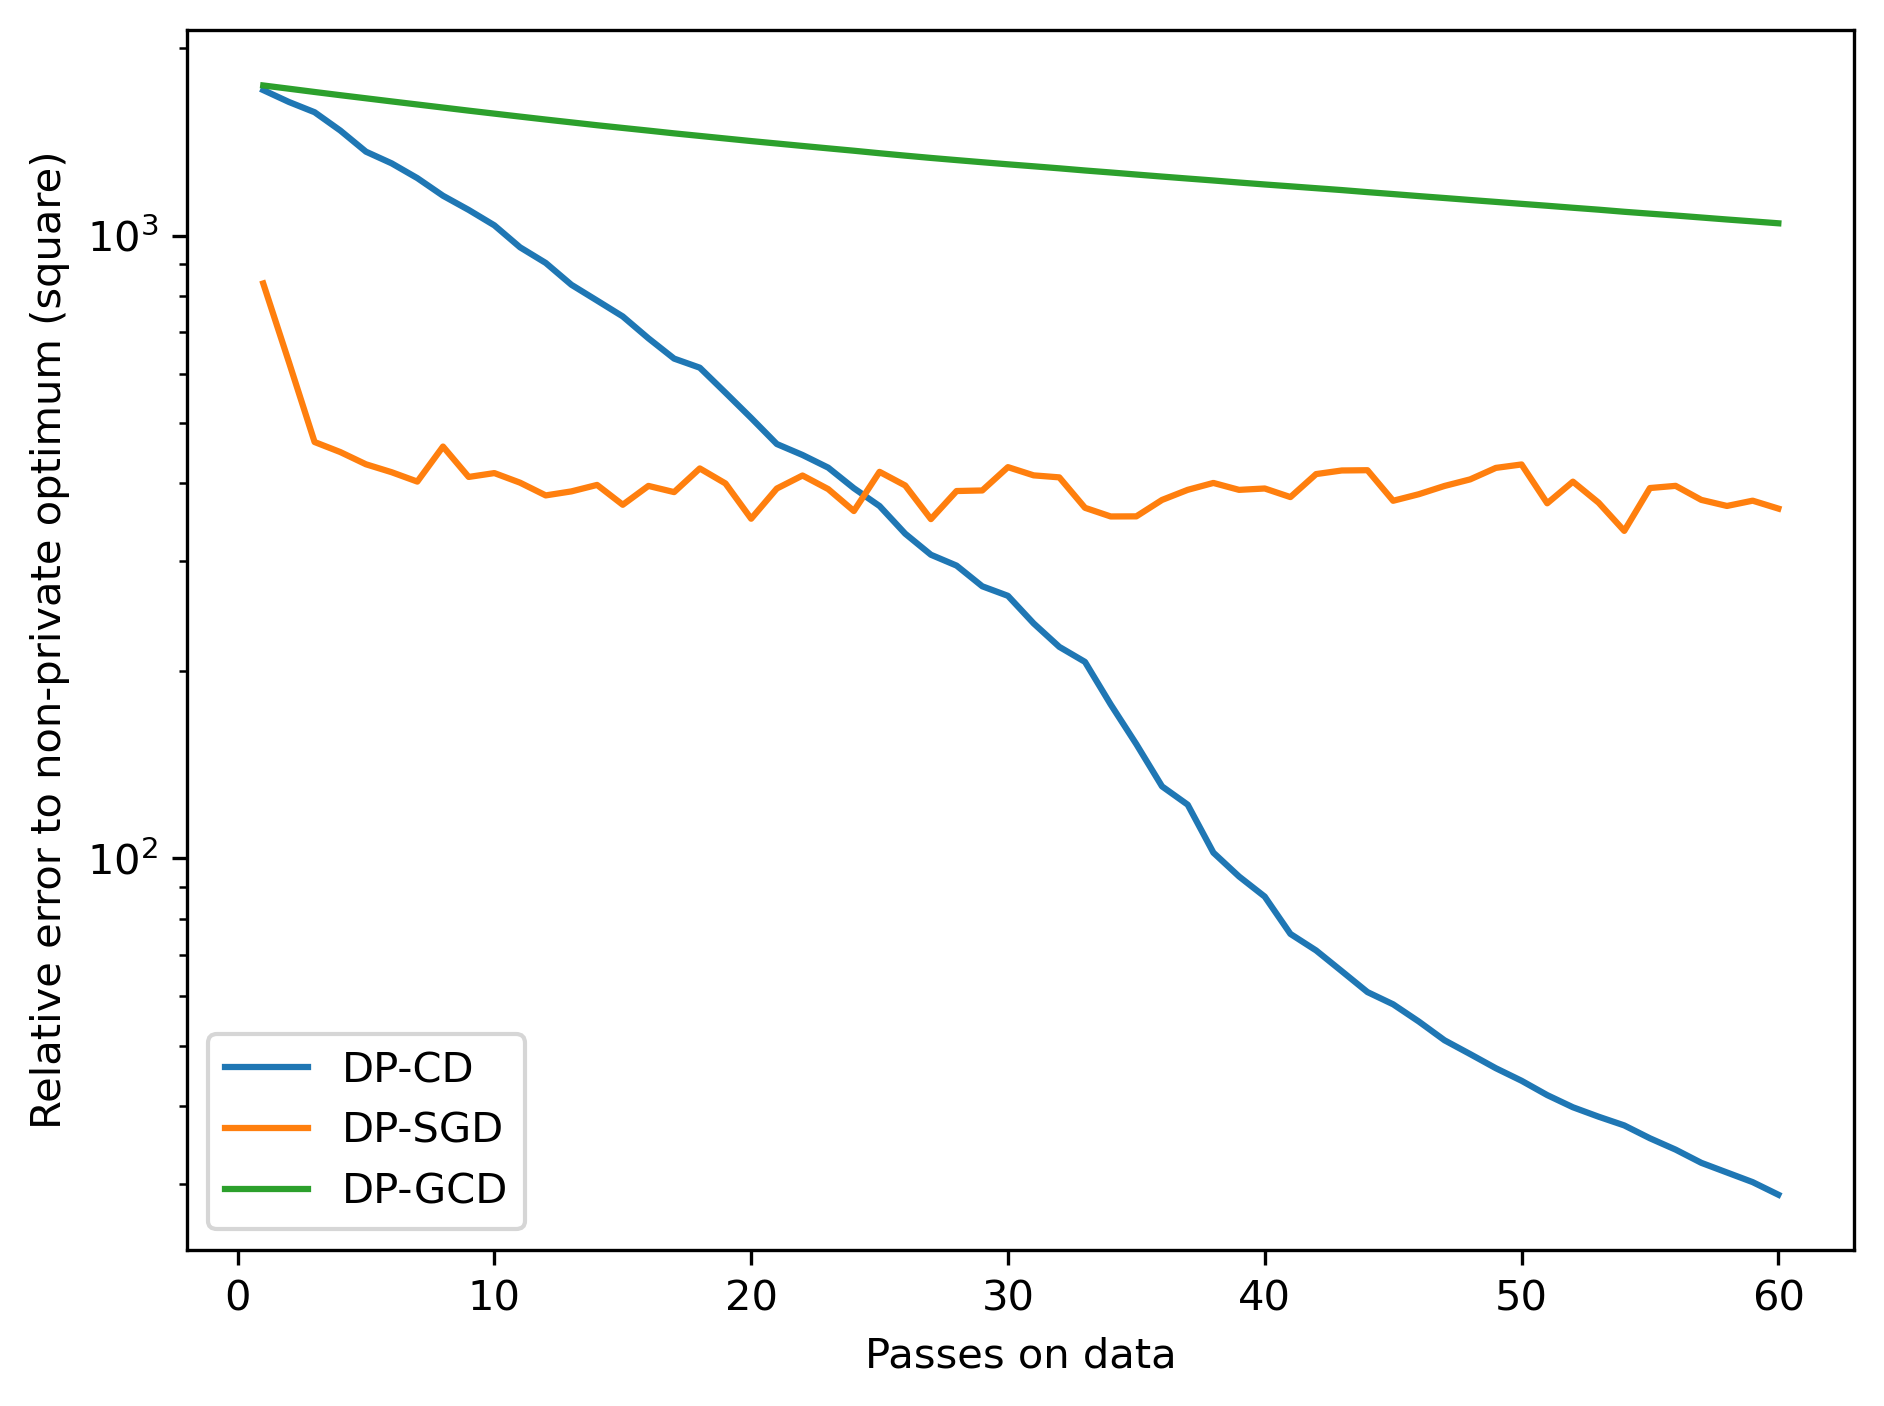
\includegraphics[width=0.85\textwidth]{square_results.png}
\end{center}

\vspace{-0.5em}

\textbf{Observation:} On $p = 1000$ with $s = 10$ non-zeros, DP-GCD dramatically outperforms. Reaches $10^{-2}$ error within 60 passes; baselines stay above $10^{-1}$.
\end{frame}

\begin{frame}{Experiment 4: California (Low-dim Regression)}
\begin{center}
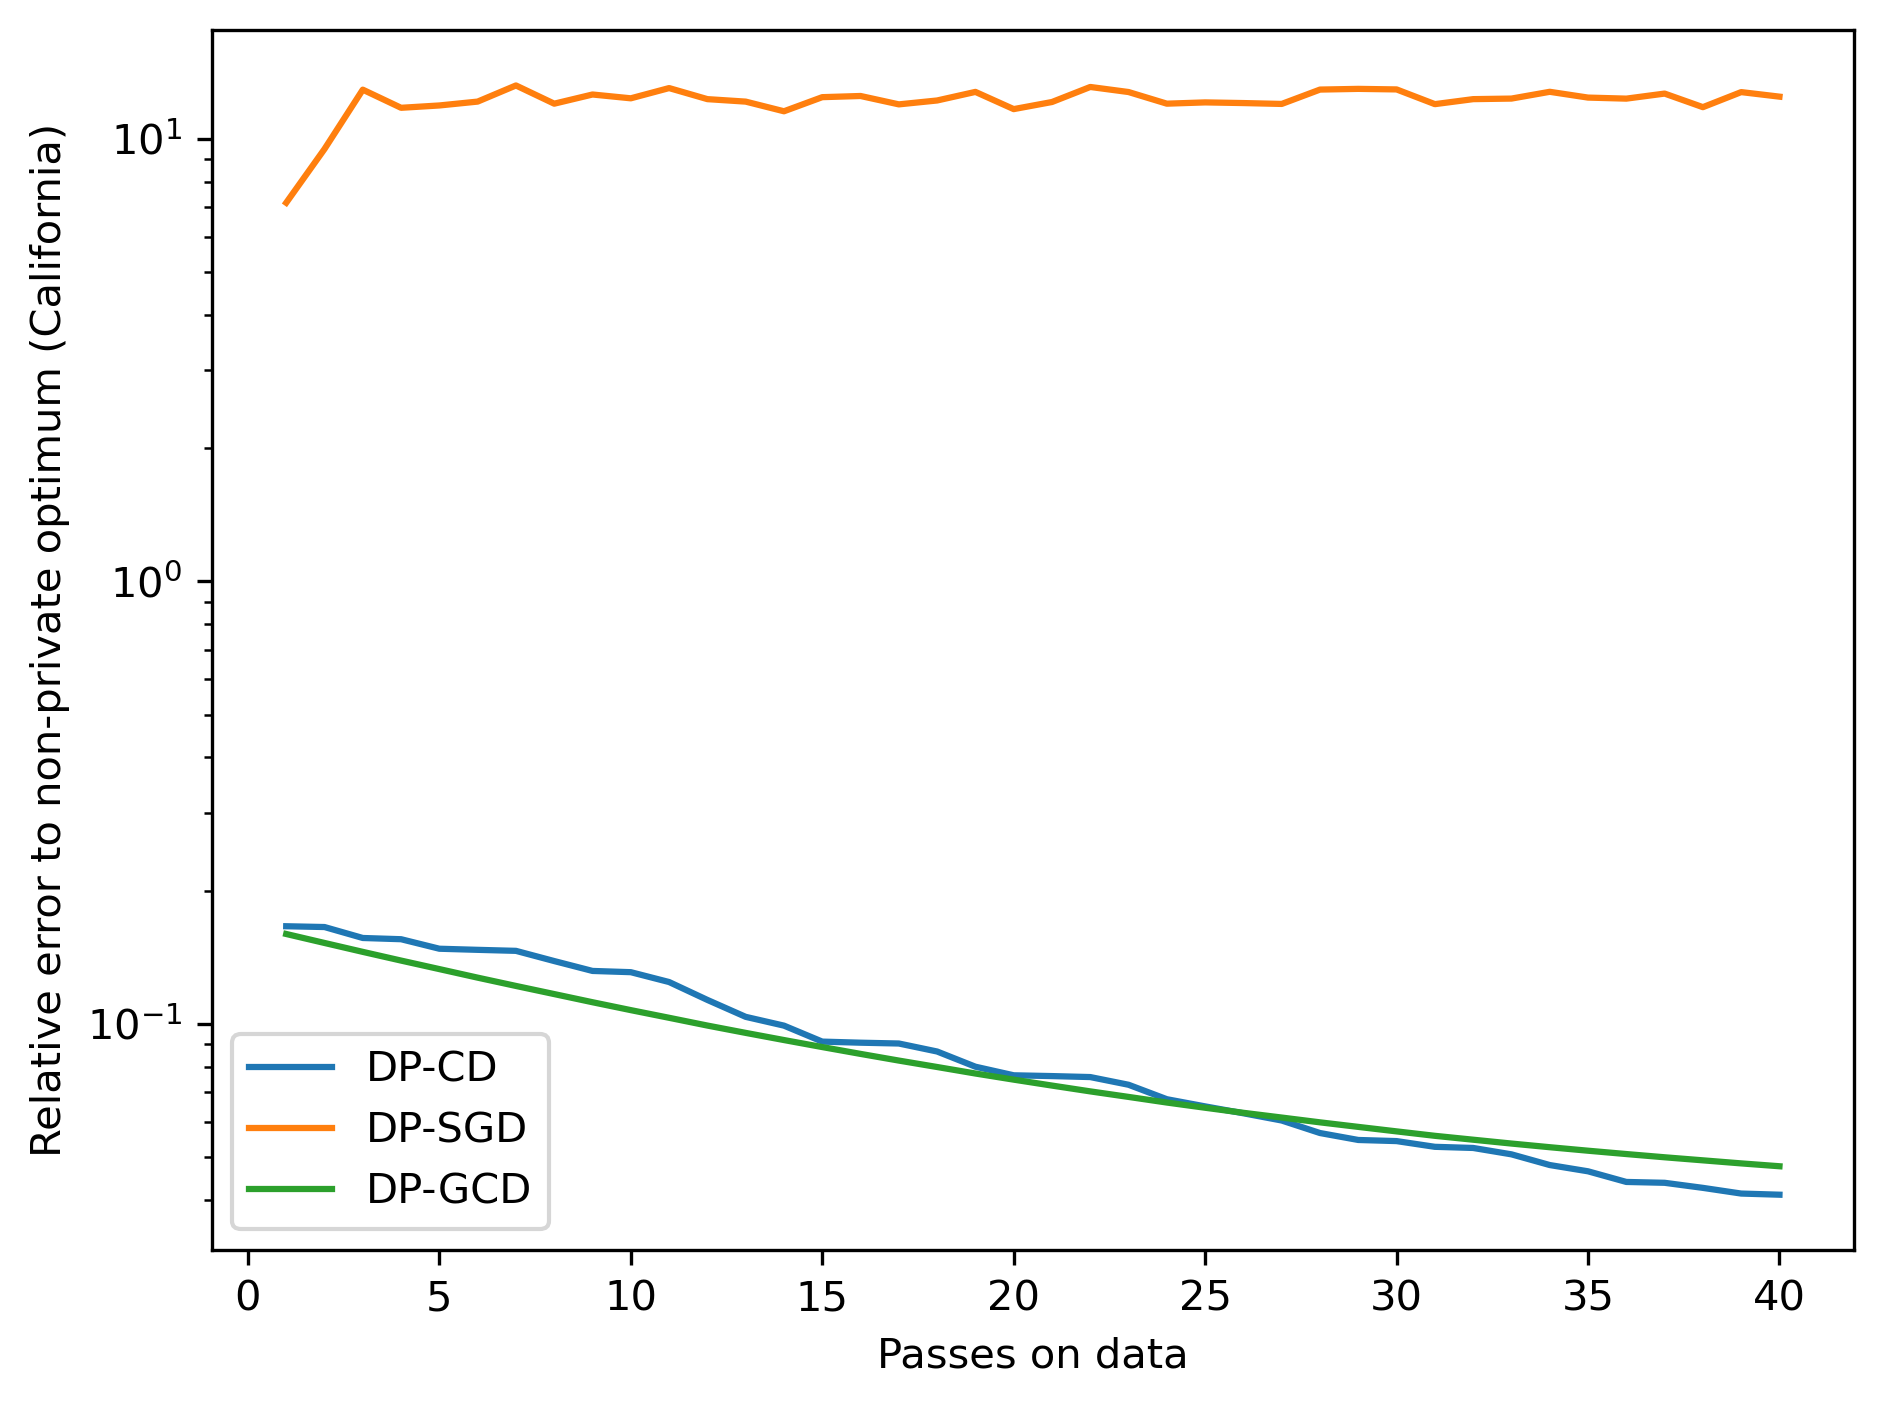
\includegraphics[width=0.85\textwidth]{california_results.png}
\end{center}

\vspace{-0.5em}

\textbf{Observation:} All three methods perform similarly on $p = 8$. DP-GCD's per-iteration overhead not justified in low dimensions without sparsity.
\end{frame}

\begin{frame}{Experiment 5: Madelon (Medium-dim Classification)}
\begin{center}
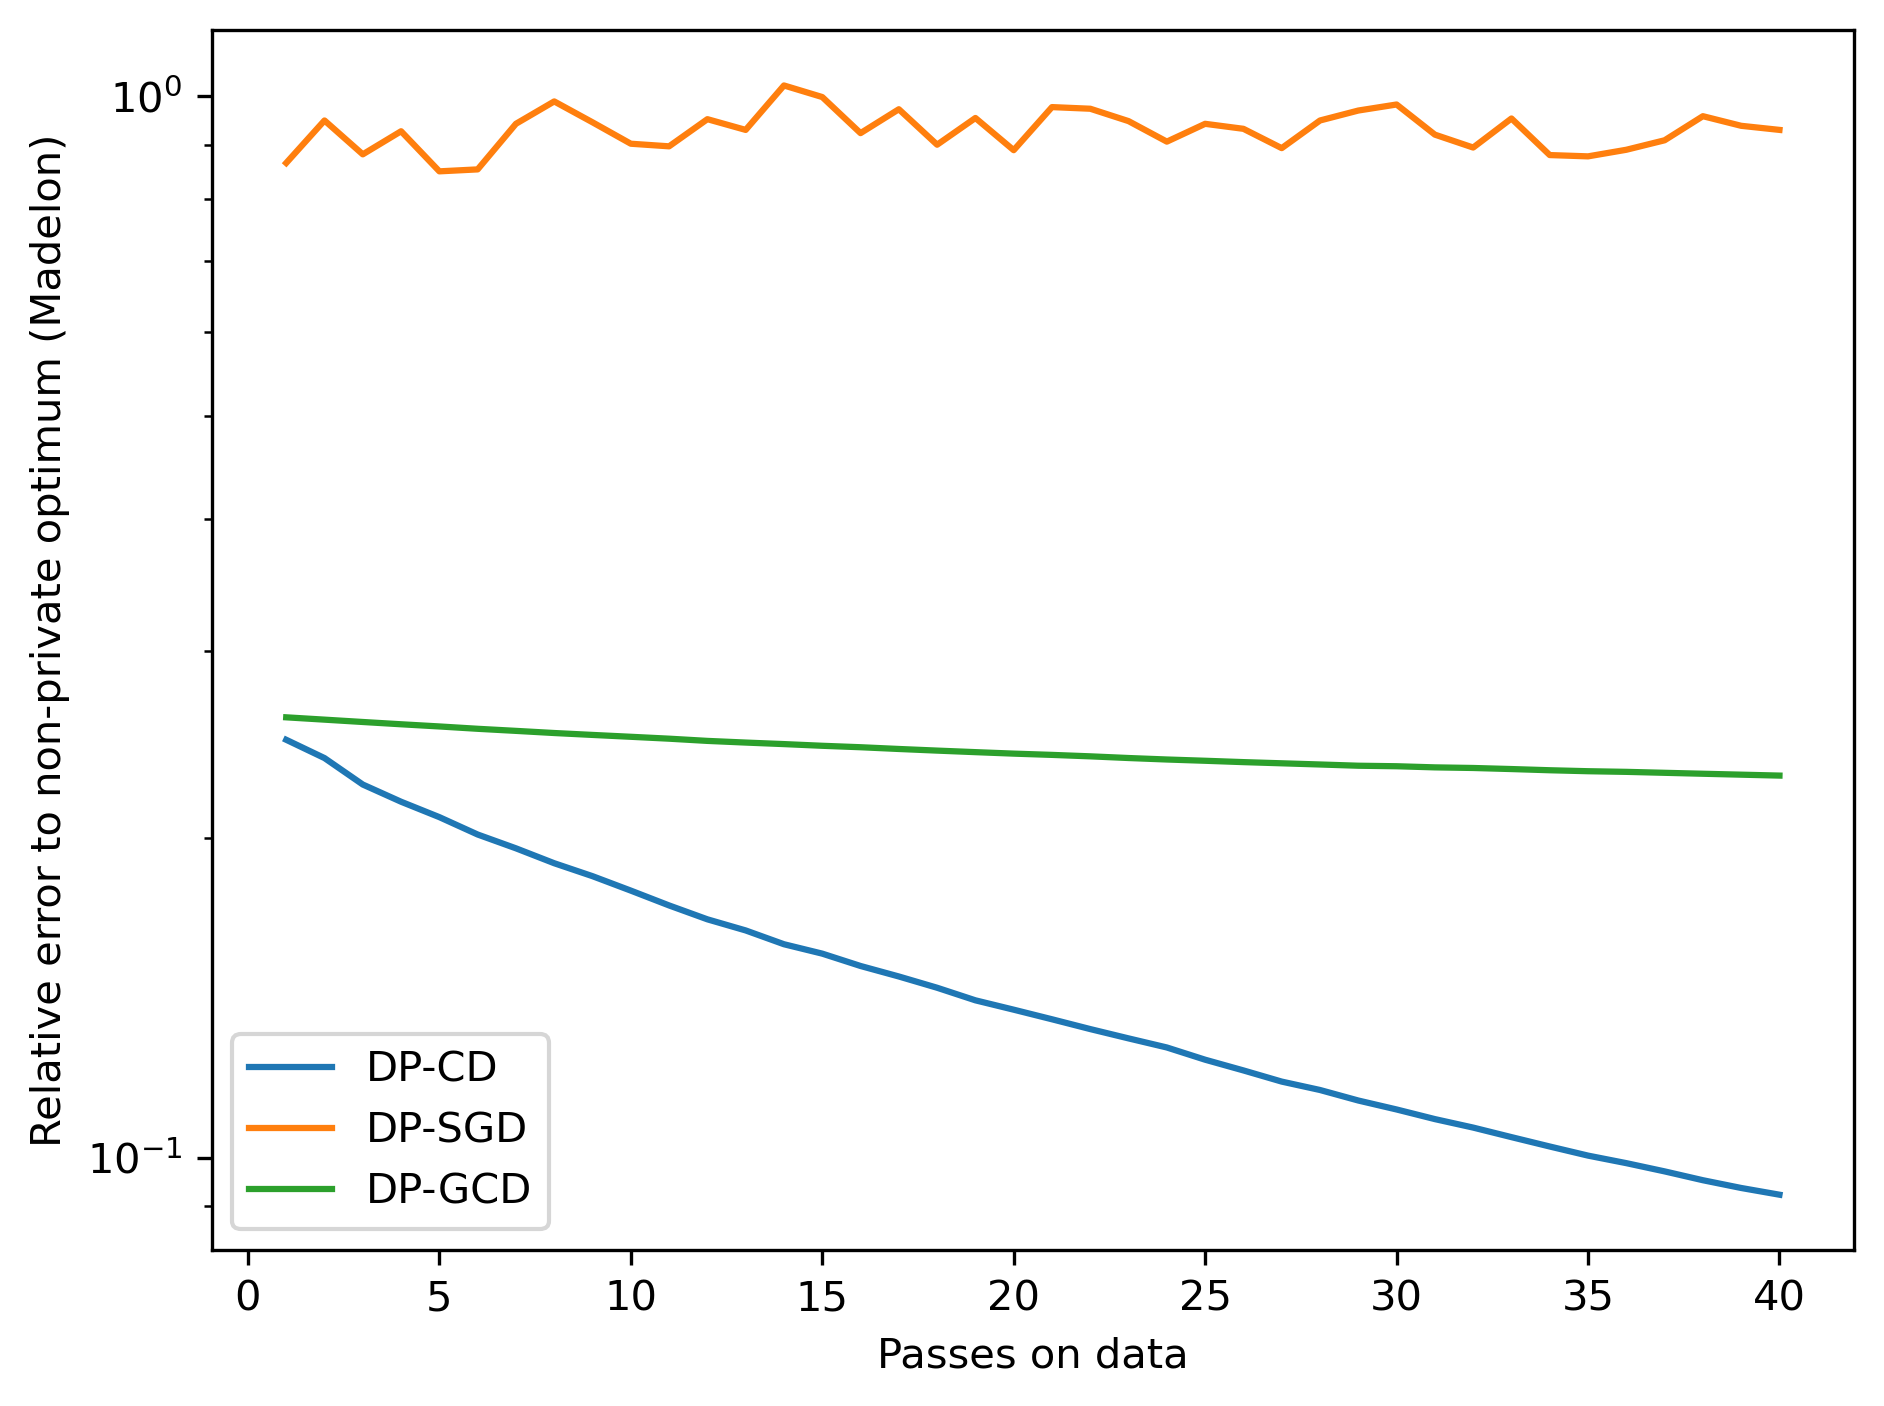
\includegraphics[width=0.85\textwidth]{madelon_results.png}
\end{center}

\vspace{-0.5em}

\textbf{Observation:} On $p = 501$, DP-GCD outperforms baselines by 2--3$\times$ in early passes. Consistent with quasi-sparse structure exploitation.
\end{frame}

\begin{frame}{Experiment 6: Dorothea-like (Very High-dim Sparse)}
\begin{center}
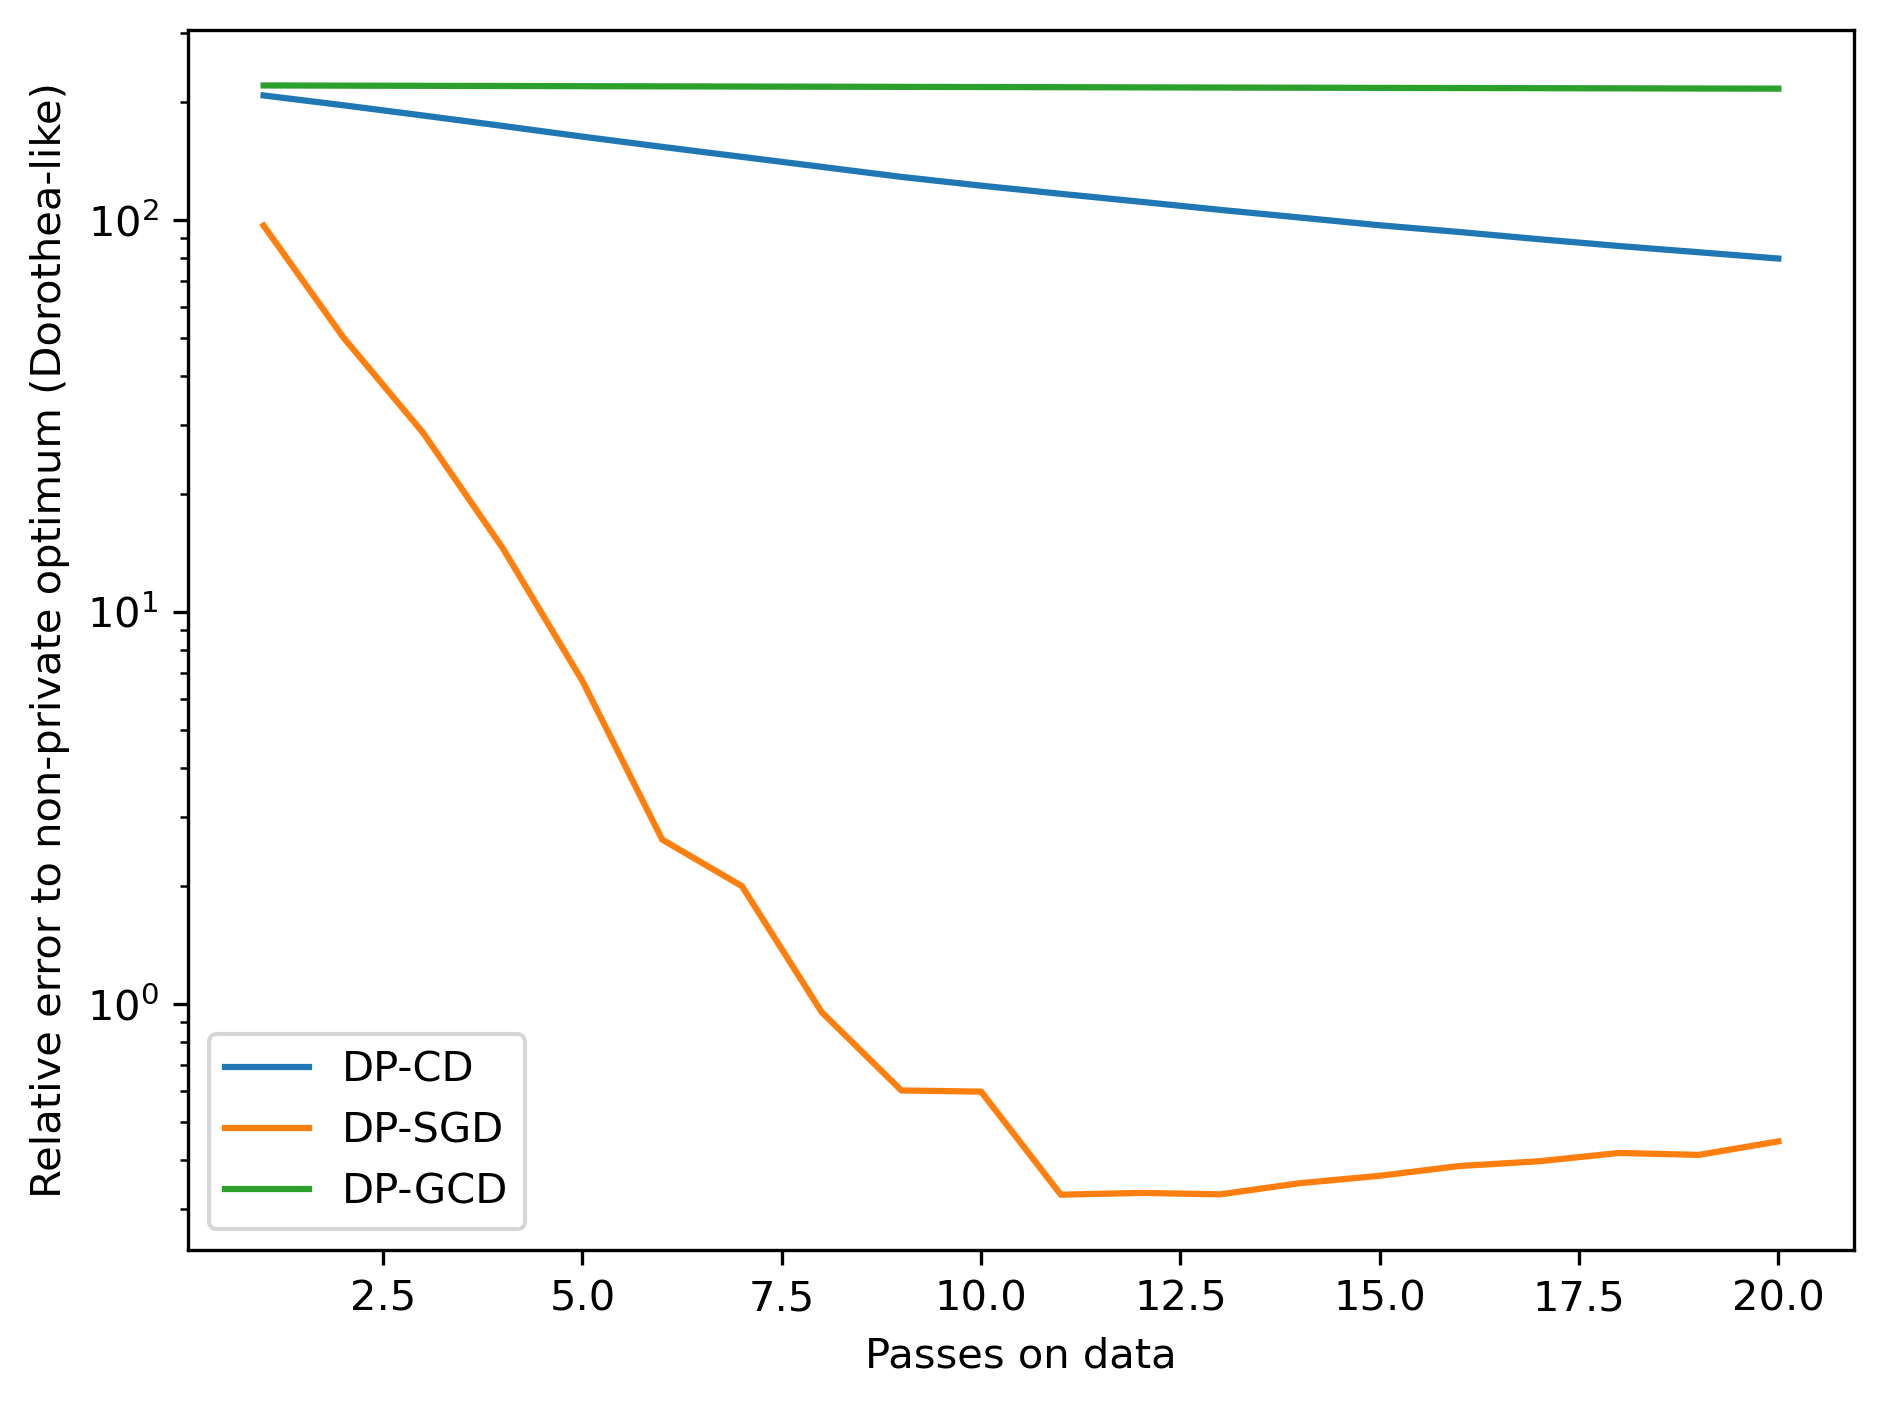
\includegraphics[width=0.85\textwidth]{dorothea_results.png}
\end{center}

\vspace{-0.5em}

\textbf{Observation:} On $p = 5000$ with $s = 50$, DP-GCD is the \alert{only method that converges}. DP-SGD/DP-CD fail to decrease objective. Demonstrates dramatic advantage in extreme high-dim regime.
\end{frame}

\begin{frame}{Key Experimental Takeaways}
\begin{enumerate}
\item \textbf{High-dim sparse (square, dorothea):} DP-GCD \alert{dramatically} outperforms ($\times 10$ or more)

\item \textbf{Quasi-sparse (log1, log2, madelon):} DP-GCD consistently 2--3$\times$ faster

\item \textbf{Low-dim (california):} All methods comparable; no advantage for DP-GCD

\item \textbf{Pattern:} DP-GCD excels precisely where quasi-sparsity + high-dim coexist
\end{enumerate}

\vspace{1em}

\begin{alertblock}{Conclusion}
Experiments validate theory: DP-GCD automatically adapts to problem structure, achieving logarithmic dimension dependence in favorable regimes.
\end{alertblock}
\end{frame}

\section{Critical Analysis}

\begin{frame}{Strengths}
\begin{enumerate}
\item \textbf{No domain constraints} — unconstrained problems (vs.\ DP-Frank-Wolfe)
\item \textbf{Automatic adaptation} — exploits quasi-sparsity without prior knowledge
\item \textbf{Logarithmic dimension} — achieves $\widetilde{O}(\log p)$ in favorable settings
\item \textbf{Coordinate-wise adaptivity} — fine-grained Lipschitz constants $L_j$
\item \textbf{Optimal strongly-convex rates} — $\widetilde{O}(\log p / n^2)$ without reductions
\item \textbf{Strong empirical validation} — dramatic improvements on high-dim problems
\end{enumerate}
\end{frame}

\begin{frame}{Limitations}
\begin{enumerate}
\item \textbf{Computational cost} — full gradient per iteration ($O(np)$)
\item \textbf{Proximal extension} — no theory for $\ell_1$ regularization
\item \textbf{Assumptions} — needs coordinate-wise smoothness/Lipschitzness constants
\item \textbf{Not uniformly optimal} — when $\ell_2$-norm bounds apply, DP-SGD may be better
\item \textbf{Privacy overhead} — Report-Noisy-Max noise hurts in low dimensions
\item \textbf{Smooth objectives only} — extensions to non-smooth remain open
\item \textbf{Theory-practice gap} — theoretical noise scales may be conservative
\end{enumerate}

\vspace{1em}

\begin{block}{When to Use DP-GCD}
High-dimensional problems with quasi-sparsity where privacy-utility trade-off matters more than wall-clock time.
\end{block}
\end{frame}

\section{Conclusion}

\begin{frame}{Summary}
\textbf{Main Contributions:}
\begin{enumerate}
\item \textbf{DP-GCD algorithm:} Greedy coordinate descent with Report-Noisy-Max
\item \textbf{Theoretical guarantees:} $\widetilde{O}(\log p)$ utility for unconstrained problems
\item \textbf{Automatic adaptation:} Exploits quasi-sparsity without prior knowledge
\item \textbf{Empirical validation:} Dramatic improvements on high-dim sparse problems
\end{enumerate}

\vspace{1em}

\begin{block}{Key Insight}
By focusing privacy budget on most informative coordinates, DP-GCD achieves logarithmic dimension dependence and automatically adapts to problem structure.
\end{block}

\vspace{1em}

\textbf{Impact:} Opens door to practical private learning in high dimensions (genomics, NLP, high-dim regression).
\end{frame}

\begin{frame}[standout]
Thank You!

\vspace{2em}

Questions?

\vspace{2em}

\small
Mangold, P., Bellet, A., Salmon, J., and Tommasi, M.\ (2023). \\
\emph{High-Dimensional Private Empirical Risk Minimization by Greedy Coordinate Descent.} AISTATS 2023.
\end{frame}

\end{document}